\documentclass[12pt,a4paper]{article}

\usepackage[default]{opensans}
\usepackage{amsfonts}
\usepackage{amsmath}
\usepackage{amssymb}
\usepackage{graphicx}
\usepackage[numbers,sort&compress]{natbib}
\usepackage{epsfig}
\usepackage[usenames,dvipsnames]{xcolor}
\usepackage{array}
\usepackage{url}
\usepackage[nottoc,numbib]{tocbibind}

\definecolor{myblue}{RGB}{25,25,112}

\usepackage[colorlinks=true
,urlcolor=myblue
%,urlcolor=black
,anchorcolor=myblue
,citecolor=myblue
,filecolor=myblue
,linkcolor=myblue
,menucolor=myblue
,linktocpage=true
,pdfproducer=medialab
,bookmarks=false]{hyperref}
%\usepackage{slashed}

\topmargin      -0.5in  % distance to headers
\headheight      0.2in  % height of header box
\headsep         0.3in  % distance to top line
\textheight      9.25in  % height of text
\footskip        0.3in  % distance from bottom line
\oddsidemargin   0.0in  % Horizontal alignment
\evensidemargin  0.0in  % Horizontal alignment
\textwidth       6.25in  % Horizontal alignment	


% Lengths ----------------------------------------------------------------------

% save parindent to a new length, originalparindent
\newlength{\originalparindent}
\setlength{\originalparindent}{\parindent}

% set parskip to bigskipamount for space between paragraphs
\setlength{\parskip}{\bigskipamount}

% set parindent to 0pt for disabling paragraph indentation
\setlength{\parindent}{0pt}





\date{}

\begin{document}

\thispagestyle{empty}

\begin{center}

\textsf{}

\vskip 1.2cm

{\LARGE \bf Fire Emergencies in Seattle}

\vskip 0.1cm

{\Large Correlations with Rain Patterns and Human Activity}
 

\vskip 0.75cm

{\bf \large S.~C.~Vargas}
%\let\thefootnote\relax\footnote{{\tt secavara@gmail.com}}\\

%\vskip 25pt

%{\em Department of Physics and Astronomy, Uppsala University, \\ Box 516, SE-751 20 Uppsala, Sweden \\}

\end{center}

\vskip 1cm


\begin{figure}[ht!]
\centering
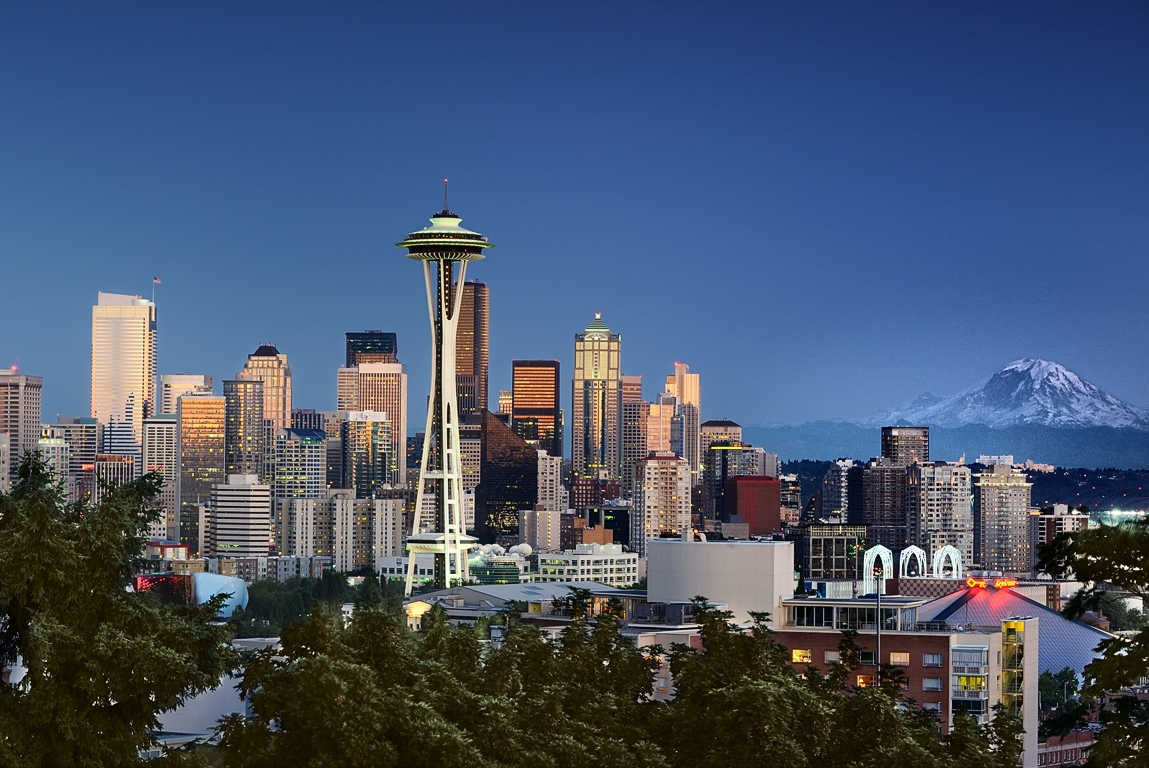
\includegraphics[scale=0.5]{Seattle_Pic.jpg}
%\caption{ }
\label{pic}
\end{figure}
\vspace{-0.8cm}
\begin{center}
{\small License notice: \href{https://www.flickr.com/people/43518209@N00}{Bala} from Seattle, USA, \href{https://commons.wikimedia.org/wiki/File:Seattle_from_Kerry_Park_(1).jpg}{Seattle from Kerry Park (1)}, \href{https://creativecommons.org/licenses/by/2.0/legalcode}{CC BY 2.0}.}
\end{center}

%\begin{center}
%{\bf ABSTRACT}\\[3ex]
%\begin{minipage}{13cm}
%\small
%This is an abstract. This is an abstract. This is an abstract. This is an abstract. This is an abstract. This is an abstract. This is an abstract. This is an abstract. This is an abstract. This is an abstract. This is an abstract. This is an abstract. This is an abstract. This is an abstract. This is an abstract. This is an abstract. This is an abstract. This is an abstract. This is an abstract. This is an abstract. This is an abstract. This is an abstract. This is an abstract. This is an abstract. This is an abstract. This is an abstract. This is an abstract. This is an abstract. This is an abstract. This is an abstract. This is an abstract. This is an abstract.
%\end{minipage}
%\end{center}

\newpage

%\tableofcontents

\section{Problem}

Can we establish trends in 911 fire calls in Seattle to predict and find patterns, or correlate them with factors such as rain patterns?

\section{Client(s)}

Governmental agencies might be interested in this study to refine strategies that pin point influential factors in the manifestation of fires in Seattle. Insurance agencies might also find this relevant. Ultimately, the objective is to reduce the significant human and financial cost generally associated with fires. Reducing the number of fires will ultimately allow the police, fire department and other dependencies to divert their resources in other issues faced by the city and its inhabitants.

\section{Sources and Data Sets}


{\large \href{https://www.kaggle.com/city-of-seattle/seattle-observed-monthly-rain-gauge-accumulations/version/16}{Seattle Observed Monthly Rain Gauge Accumulations} \cite{Daniels2018}}

These monthly data goes from October 2002 to May 2017, containing measurements of 17 rain gauges located throughout Seattle city limits. There is no information on the units describing the amounts of rain. The locations of the rain gauges are given indirectly in a image (see Figure~\ref{gauges}).

\begin{figure}[ht!]
\centering
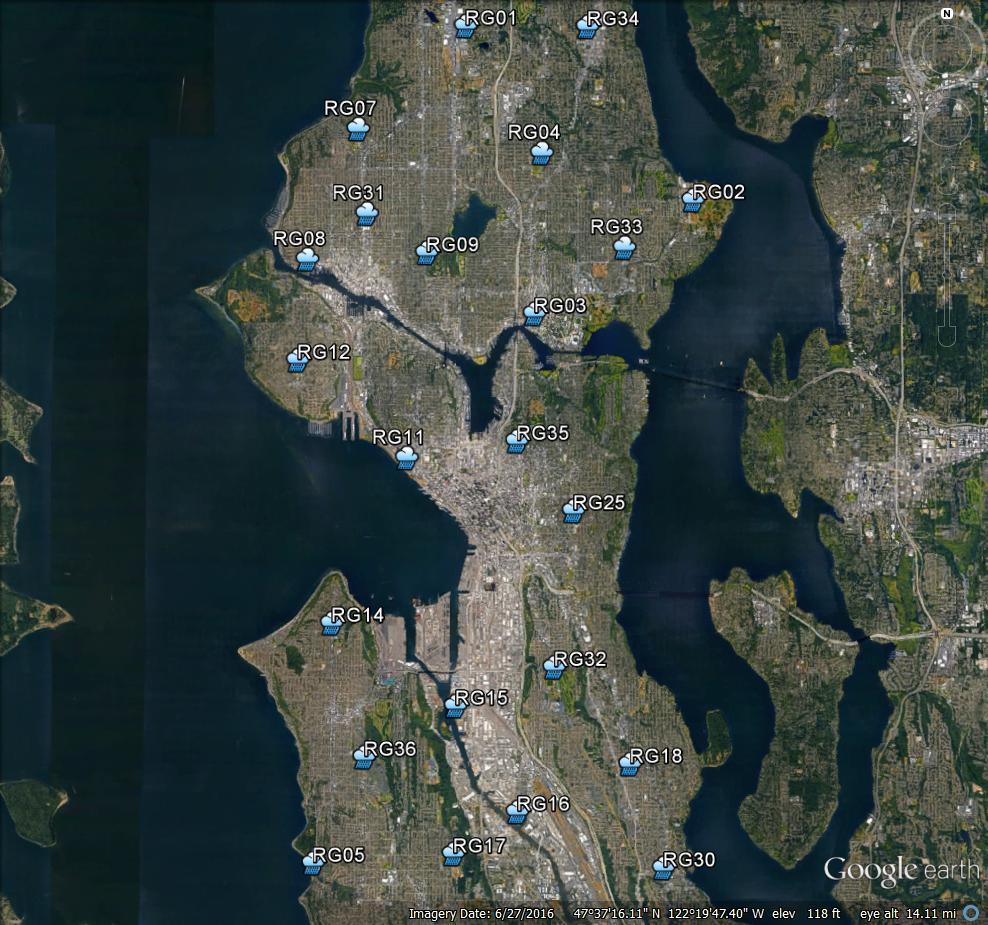
\includegraphics[scale=0.3]{SPU_DWW_RGs.jpg}
\caption{Locations of rain gauges in Seattle. In reality, measurements for only 17 of these gauges are reported. This image is part of the data set in \cite{Daniels2018}.}
\label{gauges}
\end{figure}



{\large \href{https://data.seattle.gov/Public-Safety/Seattle-Fire-911-Calls-from-3-1-2010-to-3-1-2011/d9j6-s59d}{Seattle Fire 911 Calls} \cite{FireData2018}}

Fire 911 calls from Seattle, from 2010 to 2011. It contains latitude and longitude of the location of the caller, in addition to date, time and type of call. This version corresponds to the September 2, 2018 update.

Both sets of data are freely available for download, modification and distribution, under the license \href{https://creativecommons.org/publicdomain/zero/1.0/legalcode}{CC0 1.0}.

\section{Data Wrangling and Exploratory Data Analysis}

\section{Initial Findings}

\section{Other Potentially Useful Data Sets}

%\appendix

%\section{Massive type IIA supergravity} \label{App:MIIA}

\bibliography{references}
%\bibliographystyle{plain}
\bibliographystyle{utphys}


\end{document}